%% This is file `elsarticle-template-3-num.tex',
%%
%% Copyright 2009 Elsevier Ltd
%%
%% This file is part of the 'Elsarticle Bundle'.
%% ---------------------------------------------
%%
%% It may be distributed under the conditions of the LaTeX Project Public
%% License, either version 1.2 of this license or (at your option) any
%% later version.  The latest version of this license is in
%%    http://www.latex-project.org/lppl.txt
%% and version 1.2 or later is part of all distributions of LaTeX
%% version 1999/12/01 or later.
%%
%% The list of all files belonging to the 'Elsarticle Bundle' is
%% given in the file `manifest.txt'.
%%
%% Template article for Elsevier's document class `elsarticle'
%% with numbered style bibliographic references
%%
%% $Id: elsarticle-template-3-num.tex 165 2009-10-08 07:58:10Z rishi $
%% $URL: http://lenova.river-valley.com/svn/elsbst/trunk/elsarticle-template-3-num.tex $
%%
%\documentclass[preprint,12pt]{elsarticle}

%% Use the option review to obtain double line spacing
%% \documentclass[preprint,review,12pt]{elsarticle}

%% Use the options 1p,twocolumn; 3p; 3p,twocolumn; 5p; or 5p,twocolumn
%% for a journal layout:
%% \documentclass[final,1p,times]{elsarticle}
%% \documentclass[final,1p,times,twocolumn]{elsarticle}
%% \documentclass[final,3p,times]{elsarticle}
%% \documentclass[final,3p,times,twocolumn]{elsarticle}
\documentclass[final,5p,times]{elsarticle}
%% \documentclass[final,5p,times,twocolumn]{elsarticle}

%% if you use PostScript figures in your article
%% use the graphics package for simple commands
%% \usepackage{graphics}
%% or use the graphicx package for more complicated commands
%% \usepackage{graphicx}
%% or use the epsfig package if you prefer to use the old commands
%% \usepackage{epsfig}

%% The amssymb package provides various useful mathematical symbols
\usepackage{amssymb}
%% The amsthm package provides extended theorem environments
%% \usepackage{amsthm}

%% The numcompress package shorten the last page in references.
%% `nodots' option removes dots from firstnames in references.
\usepackage[nodots]{numcompress}

%% The lineno packages adds line numbers. Start line numbering with
%% \begin{linenumbers}, end it with \end{linenumbers}. Or switch it on
%% for the whole article with \linenumbers after \end{frontmatter}.
\usepackage{lineno}

\usepackage[utf8]{inputenc}

%% Avoids linenumbers to collide with text for 5p format:
\setlength\linenumbersep{3pt}

%% natbib.sty is loaded by default. However, natbib options can be
%% provided with \biboptions{...} command. Following options are
%% valid:

%%   round  -  round parentheses are used (default)
%%   square -  square brackets are used   [option]
%%   curly  -  curly braces are used      {option}
%%   angle  -  angle brackets are used    <option>
%%   semicolon  -  multiple citations separated by semi-colon
%%   colon  - same as semicolon, an earlier confusion
%%   comma  -  separated by comma
%%   numbers-  selects numerical citations
%%   super  -  numerical citations as superscripts
%%   sort   -  sorts multiple citations according to order in ref. list
%%   sort&compress   -  like sort, but also compresses numerical citations
%%   compress - compresses without sorting
%%
%% \biboptions{comma,round}

% \biboptions{}


\journal{Computers \& Graphics}

\begin{document}

\begin{frontmatter}

%% Title, authors and addresses

%% use the tnoteref command within \title for footnotes;
%% use the tnotetext command for the associated footnote;
%% use the fnref command within \author or \address for footnotes;
%% use the fntext command for the associated footnote;
%% use the corref command within \author for corresponding author footnotes;
%% use the cortext command for the associated footnote;
%% use the ead command for the email address,
%% and the form \ead[url] for the home page:
%%
%% \title{Title\tnoteref{label1}}
%% \tnotetext[label1]{}
%% \author{Name\corref{cor1}\fnref{label2}}
%% \ead{email address}
%% \ead[url]{home page}
%% \fntext[label2]{}
%% \cortext[cor1]{}
%% \address{Address\fnref{label3}}
%% \fntext[label3]{}

\title{A Novel GPU-based Sonar Simulation for Real-Time Applications}

%% use optional labels to link authors explicitly to addresses:
%% \author[label1,label2]{<author name>}
%% \address[label1]{<address>}
%% \address[label2]{<address>}
\author[senai,ufba]{Rômulo Cerqueira}
\author[senai]{Tiago Trocoli}
\author[senai]{Gustavo Neves}
\author[ufba]{Luciano Oliveira}
\author[senai]{Sylvain Joyeux}
\author[senai,dfki]{Jan Albiez}

\address[senai]{Brazilian Institute of Robotics, SENAI CIMATEC, Salvador, Bahia, Brazil}
\address[ufba]{Intelligent Vision Research Lab, Federal University of Bahia, Salvador, Bahia, Brazil}
\address[dfki]{Robotics Innovation Center, DFKI GmbH, Bremen, Germany}

\begin{abstract}
XXXXXXXXXXXXXXXXXXXXXX
\end{abstract}

\begin{keyword}
%% keywords here, in the form: keyword \sep keyword
Synthetic Sensor Data \sep Sonar Imaging  \sep GPU-based processing \sep Robot Construction Kit (Rock) \sep Underwater Robotics.

\end{keyword}

\end{frontmatter}

%%
%% Start line numbering here if you want
%%
\linenumbers

\section{Introduction}
\label{}

% ----------------------------------------------------------------------------------

\section{Sonar Background}
\label{sonar:background}

Sonars are echo-ranging devices that use acoustic energy to locate and survey objects in a desired area underwater. The sonar's transducer emits an acoustic signal (or ping) until they hit with any object or be completely absorbed. When the ultrasonic wave collides with a surface, part of this energy is reflected and other one is refracted. Then the sonar data is built by plotting the echo measured back versus time of acoustic signal.

A single beam transmitted from a sonar is seen in Fig. XX. The horizontal and vertical beamwidths are represented by the azimuth $\theta_{B}$ and elevation $\phi_{B}$ angles respectively, where each sonar record along the beam is named bin. Since the speed of sound underwater is known or can be measured, the time axis effectively corresponds to distance from the device. The backscattered acoustic power in each bin determines the intensity value.

The array of transducer readings, with different azimuth directions, forms the final sonar image. Since all incoming signals converge on the same point, the reflected echoes could have originated anywhere along the corresponding elevation width. Therefore, the 3D information is lost in the projection into a 2D image \cite{hurtos2014b}.

Although the sonar devices address the main shortcomings of optical sensors, they present more difficult data interpretation, such as:

\begin{enumerate}[(a)]
    \item Shadowing: It is caused by objects blocking the ultrasonic waves transmission and causing regions behind them without acoustic feedback;
    \item Nonuniform resolution: The amount of pixels used to represent a record intensity grow as its range increases.
    \item Changes in viewpoint: Imaging the same scene from different viewpoints can cause occlusions, shadows movements and significant alterations of observable objects. For instance, when an outstanding object is insonified, its shadow gets shortened as the sonar becomes closer to it;
    \item Low SNR (Signal-to-Noise Ratio): The sonar suffers from low SNR mainly due the very-long-range scanning and the presence of speckle noise introduced caused by acoustic wave interferences \cite{abbott1973}.
    % \item Inhomogeneous Insonification: Since the water is a loss energy transmission medium, the farthest bins present less intensity than the closest ones.
\end{enumerate}

\subsection{Imaging Sonar Devices}

The most common types of acoustic sonars are MSIS (Mechanical Scanning Imaging Sonar) and FLS (Forward-Looking Sonar). In the first one (Fig. XX), with one beam per reading, the sonar image is built for each pulse; these images are usually shown on a display pulse by pulse, and the head position reader is rotated according to motor step angle. After a full $360^{\circ}$ sector reading (or the desired sector defined by left and right limit angles), the accumulated sonar data is overwritten. Since the vehicle is moving during the data acquisition process, a undistortion method need to be applied. This sonar device is useful for obstacle avoidance \cite{ganesan2015} and navigation \cite{ribas2010} applications.

For the FLS, with \textit{n} beams being read simultaneously, the current data is overwritten by the next one with a high framerate, similar to a streaming video imagery for real-time applications. This imaging sonar is commonly used for navigation \cite{fallon2013}, mosaicing \cite{hurtos2014a} and target tracking \cite{liu2016} approaches.
%
% The sonar reading modes are shown in Figure XX.

% \begin{figure}[h]
% \centering
% \subfigure[][]{
% 	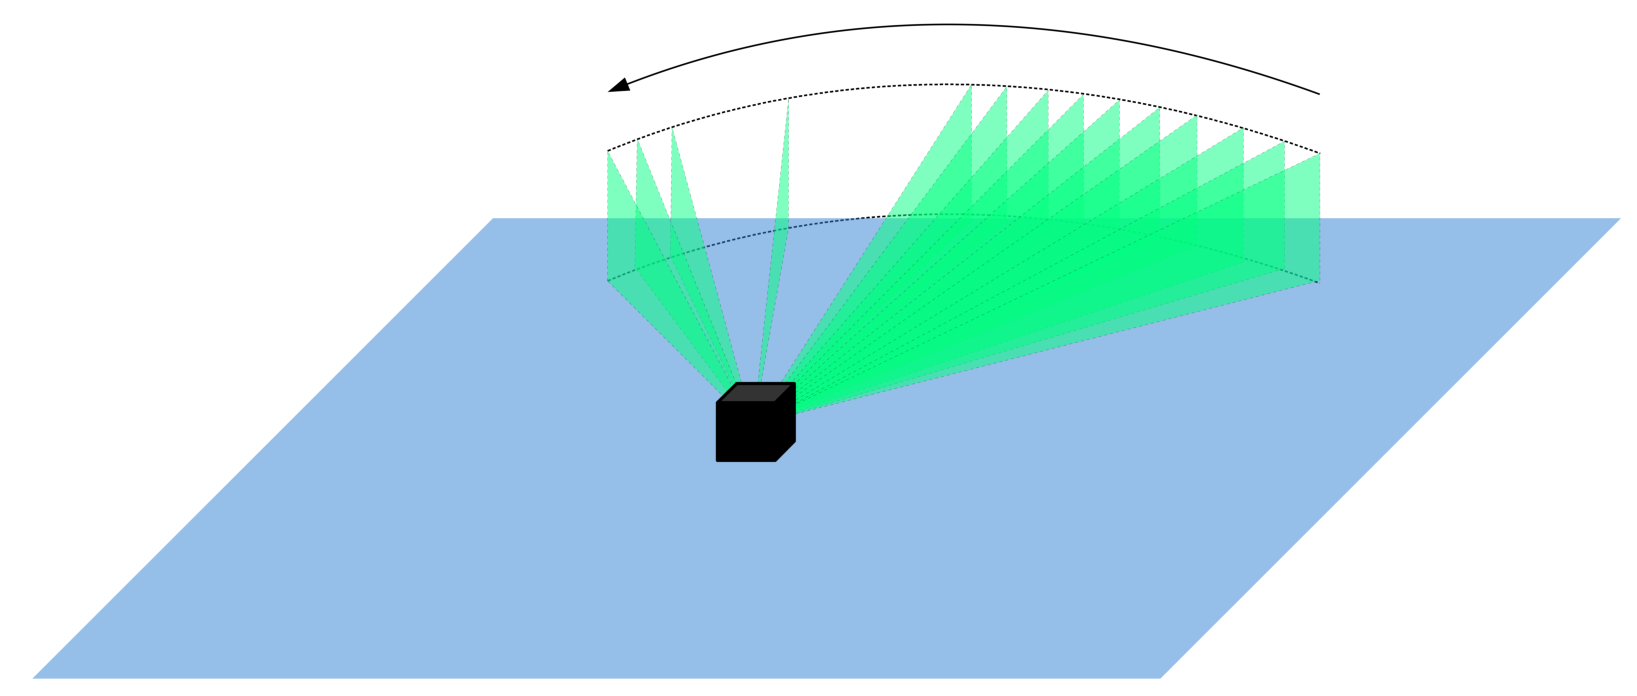
\includegraphics[width=0.47\columnwidth]{figs/sonar_swarths_msis}
%     \label{fig:swarths:msis}
% }
% \subfigure[][]{
% 	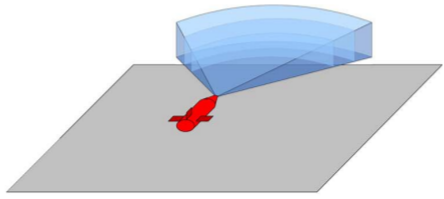
\includegraphics[width=0.45\columnwidth]{figs/sonar_swarths_fls}
%     \label{fig:swarths:fls}
% }

% Different categories of sonars exists, depending on
% frequency, transducer design and echo processing methods.
%
%
%

%

\subsection{Underwater Sonar Devices}
\label{}

% ----------------------------------------------------------------------------------

\section{Closely-related Works}
\label{}

% Several models have been used to simulate sonar data. \cite{waite2002} applied frequency-domain signal processing to generate synthetic aperture sonar image. In this method, the acoustic image was created by expressing the Fourier transform of the received signal in terms of the transmitted signal. Simplifications in the frequency domain model resulted in a basic illumination model.
%
% An application of optical ray tracing to the simulation of underwater side-scan sonar imagery was presented in \cite{bell1997}. The sonar images were generated by the use of acoustic signals represented by rays. The process of projecting rays is repeated for a 2D-array, representing all angles the sonar can emit signal. Then a 3D point cloud is constructed from the ray detection point with high computational costs.
%
% The basic methodology of 2D forward-looking sonar simulation, using optical ray tracing combined with processing in the frequency domain, was proposed in \cite{sac2015}. The average simulation time of $2.5$ minutes for one simulated image prevents its evaluation in real time.
%
% In \cite{demarco2015}, a 2D forward-looking sonar was proposed using acoustic tubes instead of rays. This implementation added noise to the point cloud generated by rays before converting it into a sonar image, but the material reflectance was statically defined. It resulted in same intensity values for all points on a single object.
%
% We are not aware of any previous work which customizes the 3D rendering pipeline to generate underwater sonar images -- the present work therefore represents an important innovation in sonar simulation. Another contribution is that the method proposed herein is able to reproduce any type of underwater sonar images, as seen in evaluation tests with two kind of simulated sonars.

% ----------------------------------------------------------------------------------

\section{GPU-based Sonar Simulation Modeling}
\label{dev}

The goal of this work is to simulate any kind of underwater sonar by vertex and fragment processing, with a low computational-time cost. The complete pipeline of this implementation, from the virtual scene to the synthetic acoustic image, is seen in Fig. XX and detailed in the following subsections. The sonar simulation is written in C++ with OpenCV~\footnote{http://opencv.org/} support as ROCK~\footnote{http://rock-robotics.org/} packages.

\subsection{Underwater Environment}
\label{dev:uwscene}

The Rock-Gazebo integration \cite{watanabe2015} provides the underwater scenario and allows real-time Hardware-in-the-Loop simulations, where Gazebo handles the physical engines and the Rock's graphics tools are responsible by the scene visualization. The graphical data in Rock are based on OpenSceneGraph~\footnote{http://www.openscenegraph.org/} library, a open source C/C++ 3D graphics toolkit built on OpenGL. The osgOcean~\footnote{http://wiki.ros.org/osgOcean} library is used to simulate the ocean's visual effects, and the ocean buoyancy is defined by the Gazebo plugin as described in \cite{watanabe2015}.

All scene's aspects, such as terrain, robot parts (including sensors and joints) and others objects presented in the environment, are defined by SDF files, which uses the SDFormat~\footnote{http://sdformat.org}, a XML format used to describe simulated models and environments.

Each component described in the SDF file becomes a ROCK component, which is based on the Orocos RTT (Real Time Toolkit)~\footnote{http://www.orocos.org/rtt} and provides ports, properties and operations as its communication layer. When the models are loaded, ROCK-Gazebo creates ports to allow other system components to interact with the simulated models \cite{cerqueira2016}.

\subsection{Shader Rendering}
\label{dev:shader}
% Talk about the orthographic camera here

Shaders run on the graphic card and allow to take full control of the rendering pipeline process. The OpenGL Shading Language (GLSL)~\footnote{https://www.opengl.org/documentation/glsl/} is a high-level language with a C-based syntax which handles the graphics pipeline on the GPU (Graphics Processing Unit). In order to simulate the sonar sensoring, the fragment and vertex shaders are designed as a camera in an orthographic projection, with a desired position, orientation and field of view. Then the 2D sonar data is computed as:

\begin{itemize}
    \item \textit{Depth} is the camera focal length and is calculated by the euclidean distance to object's surface point;
    \item \textit{Intensity} presents the echo reflection energy based on an object's surface normal.
\end{itemize}

Most real-world surfaces present irregularities and different reflectances. For more realistic sensing, the normal data can also defined by bump mapping and material properties. Bump mapping is a normal-perturbation rendering technique to simulate bumps and wrinkles on the object's surface by passing textures and modifying the normal directions. It is much faster and consumes less resources for the same level of detail compared to displacement mapping, because the geometry remains unchanged. Since bump maps are built in tangent space, interpolating the normal vertex and the texture, a TBN(tangent, bitangent and normal) matrix is used to convert the normal values to world space.

% Since bump maps are built in tangent space, inteporlating the normal vertex and the texture,

% Both intensity and depth data are normalized in the [0,1] interval.

% These data are normalized between $0.0$ and $1.0$, where means, respectively, no echo energy and maximum echo energy for intensity data. For depth data, the minimum value portrays a close object while the maximum value represents a far object, limited by sonar max range. Angle distortion has $0.0$ value in center column, and $1.0$ value in both border columns which presents FOV-X half value. At the end, the shader process gives a 3-channel matrix data of intensity, depth and angle distortion stored in each channel.

% Talk about bump mapping (+ TBN Matrix) and material properties here

% Bump mapping is a texturebased
% rendering approach for simulating lighting effects
% caused by patterned irregularities on otherwise locally smooth
% surfaces. By encoding such surface patterns in texture maps,
% bump mapping simulates a surface’s irregular lighting
% appearance without the complexity and expense of modeling
% the patterns as true geometric perturbations to the surface.
% Bump mapping combines per-fragment lighting with
% surface normal perturbations supplied by a texture, in order to
% simulate lighting interactions on bumpy surfaces. This effect is
% achieved without requiring excessive geometric tessellation of
% the surface. As an example, bump mapping can be used to
% makes surfaces appear as if they have bricks protruding from
% them, and mortar between the bricks.
% Most real-world surfaces such as brick walls or cobblestones
% have small-scale bumpy features that are too fine to
% represent with highly tessellated geometry

\subsection{Synthetic Sonar Data}
\label{dev:sonardata}

The 3-channel matrix is processed in order to simulate the virtual sonar data. Initially the matrix is splitted in beam parts. The angular distortion is radially spaced over the horizontal field of view, so each column is correlated with its respective beam, according to sonar bearings, as seen in Fig. \ref{fig:sonar_sim}.

Each beam sub-image (with its respective columns) is converted into bin intensities using the depth and intensity values from shader process. In a real sonar, the bin number is proportional to the real distance from the sensor. In other words, the initial bins represent the closest distances, while the latest bins are the furthest ones. Therefore, a depth histogram is evaluated to associate each pixel with its respective bin, according to the depth channel. This information is used to calculate the intensity of each bin.

Due to acoustic attenuation in the water, the final bins have less echo strength than the first ones, because energy is lost in the environment. In order to correct for this, the sonar uses an energy normalization that applies a time varying gain to spreading losses in the bins. In this simulation approach, the accumulated intensity in each bin is normalized as
\begin{equation}
    \label{eq:1}
    I_{bin} = \sum\limits_{x=1}^n \frac{1}{n} \times S(i_{x}) \, ,
\end{equation}
where $I_{bin}$ is the accumulated intensity in the bin after the energy normalization, $x$ is the pixel in the shader matrix, $n$ is the depth histogram value (number of pixels) of that bin, $S(i_{x})$ is the sigmoid function and $i_{x}$ is the intensity value of the pixel $x$.

Finally, the shader image resolution needs to be big enough to fill all bins. If the number of bins is greater than 750, the depth histogram will contain some blank spaces that will reflect in the final sonar image as "black holes". To avoid this problem, it is necessary to distribute the sonar intensity data by applying a simple linear interpolation.

\subsection{Noise Model}
\label{dev:noise}

Imaging sonar systems are perturbed by a multiplicative noise known as speckle. It is caused by coherent processing of backscattered signals from multiple distributed targets, that degrades image quality and the visual evaluation. The noisy image has been expressed as \cite{lee1980}:

\begin{equation}
\label{eq:2}
y(t) = x(t) \times n(t) \, ,
\end{equation}

where $t$ is the time instant, $y(t)$ is the noised image, $x(t)$ is the free-noise image and $n(t)$ is the speckle noise matrix. This kind of noise is well-modeled as a Gaussian distribution. The physical explanation is provided by the Central Limit of Theorem, which states that the sum of many independent and identically distributed random variables tends to behave a Gaussian random variable \cite{papoulis2002}. For a more realistic sensing, a Gaussian distribution is built and applied as speckle noise in the simulated sonar image. After that, the simulation sonar data process is done.

\subsection{ROCK's Sonar Structure}
\label{}

To export and display the sonar image, the simulated data is encapsulated as ROCK's sonar data type and provided as an output port of ROCK's component.


% ----------------------------------------------------------------------------------

\section{Results and Discussion}
\label{}

% ----------------------------------------------------------------------------------

\section{Conclusion and Outlook}
\label{}

%% The Appendices part is started with the command \appendix;
%% appendix sections are then done as normal sections
%% \appendix

%% \section{}
%% \label{}

%% References
%%
%% Following citation commands can be used in the body text:
%% Usage of \cite is as follows:
%%   \cite{key}          ==>>  [#]
%%   \cite[chap. 2]{key} ==>>  [#, chap. 2]
%%   \citet{key}         ==>>  Author [#]

%% References with bibTeX database:

\nocite{*}
\bibliographystyle{model3-num-names}
\bibliography{elsarticle-template-3-num}

%% Authors are advised to submit their bibtex database files. They are
%% requested to list a bibtex style file in the manuscript if they do
%% not want to use model3-num-names.bst.

%% References without bibTeX database:

% \begin{thebibliography}{00}

%% \bibitem must have the following form:
%%   \bibitem{key}...
%%

% \bibitem{}

% \end{thebibliography}


\end{document}

%%
%% End of file `elsarticle-template-3-num.tex'.
